\documentclass[a4paper]{article}
\usepackage[utf8]{inputenc}
\usepackage[spanish, es-tabla]{babel}

\usepackage{amsmath}
\usepackage{amsfonts}
\usepackage{amssymb}

\usepackage{float}
\usepackage{graphicx}
\graphicspath{ {./Imagenes/} }

\usepackage{multirow}
\setlength{\doublerulesep}{\arrayrulewidth}

\usepackage{tikz}
\usetikzlibrary{matrix,calc}

\usepackage{array}
\newcolumntype{C}[1]{>{\centering\let\newline\\\arraybackslash\hspace{0pt}}m{#1}}

\usepackage[american]{circuitikz}

\usepackage{fancyhdr}

\usepackage{units} 

\pagestyle{fancy}
\fancyhf{}
\lhead{22.13 Electrónica III}
\rhead{Mechoulam, Lambertucci, Martorel, Londero}
\rfoot{Página \thepage}

\usepackage{tikz}
\usetikzlibrary{matrix,calc}

%isolated term
%#1 - Optional. Space between node and grouping line. Default=0
%#2 - node
%#3 - filling color
\newcommand{\implicantsol}[3][0]{
    \draw[rounded corners=3pt, fill=#3, opacity=0.3] ($(#2.north west)+(135:#1)$) rectangle ($(#2.south east)+(-45:#1)$);
    }


%internal group
%#1 - Optional. Space between node and grouping line. Default=0
%#2 - top left node
%#3 - bottom right node
%#4 - filling color
\newcommand{\implicant}[4][0]{
    \draw[rounded corners=3pt, fill=#4, opacity=0.3] ($(#2.north west)+(135:#1)$) rectangle ($(#3.south east)+(-45:#1)$);
    }

%group lateral borders
%#1 - Optional. Space between node and grouping line. Default=0
%#2 - top left node
%#3 - bottom right node
%#4 - filling color
\newcommand{\implicantcostats}[4][0]{
    \draw[rounded corners=3pt, fill=#4, opacity=0.3] ($(rf.east |- #2.north)+(90:#1)$)-| ($(#2.east)+(0:#1)$) |- ($(rf.east |- #3.south)+(-90:#1)$);
    \draw[rounded corners=3pt, fill=#4, opacity=0.3] ($(cf.west |- #2.north)+(90:#1)$) -| ($(#3.west)+(180:#1)$) |- ($(cf.west |- #3.south)+(-90:#1)$);
}

%group top-bottom borders
%#1 - Optional. Space between node and grouping line. Default=0
%#2 - top left node
%#3 - bottom right node
%#4 - filling color
\newcommand{\implicantdaltbaix}[4][0]{
    \draw[rounded corners=3pt, fill=#4, opacity=0.3] ($(cf.south -| #2.west)+(180:#1)$) |- ($(#2.south)+(-90:#1)$) -| ($(cf.south -| #3.east)+(0:#1)$);
    \draw[rounded corners=3pt, fill=#4, opacity=0.3] ($(rf.north -| #2.west)+(180:#1)$) |- ($(#3.north)+(90:#1)$) -| ($(rf.north -| #3.east)+(0:#1)$);
}

%group corners
%#1 - Optional. Space between node and grouping line. Default=0
%#2 - filling color
\newcommand{\implicantcantons}[2][0]{
    \draw[rounded corners=3pt, opacity=.3] ($(rf.east |- 0.south)+(-90:#1)$) -| ($(0.east |- cf.south)+(0:#1)$);
    \draw[rounded corners=3pt, opacity=.3] ($(rf.east |- 8.north)+(90:#1)$) -| ($(8.east |- rf.north)+(0:#1)$);
    \draw[rounded corners=3pt, opacity=.3] ($(cf.west |- 2.south)+(-90:#1)$) -| ($(2.west |- cf.south)+(180:#1)$);
    \draw[rounded corners=3pt, opacity=.3] ($(cf.west |- 10.north)+(90:#1)$) -| ($(10.west |- rf.north)+(180:#1)$);
    \fill[rounded corners=3pt, fill=#2, opacity=.3] ($(rf.east |- 0.south)+(-90:#1)$) -|  ($(0.east |- cf.south)+(0:#1)$) [sharp corners] ($(rf.east |- 0.south)+(-90:#1)$) |-  ($(0.east |- cf.south)+(0:#1)$) ;
    \fill[rounded corners=3pt, fill=#2, opacity=.3] ($(rf.east |- 8.north)+(90:#1)$) -| ($(8.east |- rf.north)+(0:#1)$) [sharp corners] ($(rf.east |- 8.north)+(90:#1)$) |- ($(8.east |- rf.north)+(0:#1)$) ;
    \fill[rounded corners=3pt, fill=#2, opacity=.3] ($(cf.west |- 2.south)+(-90:#1)$) -| ($(2.west |- cf.south)+(180:#1)$) [sharp corners]($(cf.west |- 2.south)+(-90:#1)$) |- ($(2.west |- cf.south)+(180:#1)$) ;
    \fill[rounded corners=3pt, fill=#2, opacity=.3] ($(cf.west |- 10.north)+(90:#1)$) -| ($(10.west |- rf.north)+(180:#1)$) [sharp corners] ($(cf.west |- 10.north)+(90:#1)$) |- ($(10.west |- rf.north)+(180:#1)$) ;
}

%Empty Karnaugh map 4x4
\newenvironment{Karnaugh}%
{
\begin{tikzpicture}[baseline=(current bounding box.north),scale=0.8]
\draw (0,0) grid (4,4);
\draw (0,4) -- node [pos=0.7,above right,anchor=south west] {ba} node [pos=0.7,below left,anchor=north east] {dc} ++(135:1);
%
\matrix (mapa) [matrix of nodes,
        column sep={0.8cm,between origins},
        row sep={0.8cm,between origins},
        every node/.style={minimum size=0.3mm},
        anchor=8.center,
        ampersand replacement=\&] at (0.5,0.5)
{
                       \& |(c00)| 00         \& |(c01)| 01         \& |(c11)| 11         \& |(c10)| 10         \& |(cf)| \phantom{00} \\
|(r00)| 00             \& |(0)|  \phantom{0} \& |(1)|  \phantom{0} \& |(3)|  \phantom{0} \& |(2)|  \phantom{0} \&                     \\
|(r01)| 01             \& |(4)|  \phantom{0} \& |(5)|  \phantom{0} \& |(7)|  \phantom{0} \& |(6)|  \phantom{0} \&                     \\
|(r11)| 11             \& |(12)| \phantom{0} \& |(13)| \phantom{0} \& |(15)| \phantom{0} \& |(14)| \phantom{0} \&                     \\
|(r10)| 10             \& |(8)|  \phantom{0} \& |(9)|  \phantom{0} \& |(11)| \phantom{0} \& |(10)| \phantom{0} \&                     \\
|(rf) | \phantom{00}   \&                    \&                    \&                    \&                    \&                     \\
};
}%
{
\end{tikzpicture}
}

%Empty Karnaugh map 2x4
\newenvironment{Karnaughvuit}%
{
\begin{tikzpicture}[baseline=(current bounding box.north),scale=0.8]
\draw (0,0) grid (4,2);
\draw (0,2) -- node [pos=0.7,above right,anchor=south west] {bc} node [pos=0.7,below left,anchor=north east] {a} ++(135:1);
%
\matrix (mapa) [matrix of nodes,
        column sep={0.8cm,between origins},
        row sep={0.8cm,between origins},
        every node/.style={minimum size=0.3mm},
        anchor=4.center,
        ampersand replacement=\&] at (0.5,0.5)
{
                      \& |(c00)| 00         \& |(c01)| 01         \& |(c11)| 11         \& |(c10)| 10         \& |(cf)| \phantom{00} \\
|(r00)| 0             \& |(0)|  \phantom{0} \& |(1)|  \phantom{0} \& |(3)|  \phantom{0} \& |(2)|  \phantom{0} \&                     \\
|(r01)| 1             \& |(4)|  \phantom{0} \& |(5)|  \phantom{0} \& |(7)|  \phantom{0} \& |(6)|  \phantom{0} \&                     \\
|(rf) | \phantom{00}  \&                    \&                    \&                    \&                    \&                     \\
};
}%
{
\end{tikzpicture}
}

%Empty Karnaugh map 2x2
\newenvironment{Karnaughquatre}%
{
\begin{tikzpicture}[baseline=(current bounding box.north),scale=0.8]
\draw (0,0) grid (2,2);
\draw (0,2) -- node [pos=0.7,above right,anchor=south west] {b} node [pos=0.7,below left,anchor=north east] {a} ++(135:1);
%
\matrix (mapa) [matrix of nodes,
        column sep={0.8cm,between origins},
        row sep={0.8cm,between origins},
        every node/.style={minimum size=0.3mm},
        anchor=2.center,
        ampersand replacement=\&] at (0.5,0.5)
{
          \& |(c00)| 0          \& |(c01)| 1  \\
|(r00)| 0 \& |(0)|  \phantom{0} \& |(1)|  \phantom{0} \\
|(r01)| 1 \& |(2)|  \phantom{0} \& |(3)|  \phantom{0} \\
};
}%
{
\end{tikzpicture}
}

%Defines 8 or 16 values (0,1,X)
\newcommand{\contingut}[1]{%
\foreach \x [count=\xi from 0]  in {#1}
     \path (\xi) node {\x};
}

%Places 1 in listed positions
\newcommand{\minterms}[1]{%
    \foreach \x in {#1}
        \path (\x) node {1};
}

%Places 0 in listed positions
\newcommand{\maxterms}[1]{%
    \foreach \x in {#1}
        \path (\x) node {0};
}

%Places X in listed positions
\newcommand{\indeterminats}[1]{%
    \foreach \x in {#1}
        \path (\x) node {X};
}

% \begin{document}
%     \begin{Karnaugh}
%         \contingut{0,0,0,0,0,0,0,0,0,0,0,0,0,0,0,0}
%        \implicant{0}{2}{red}
%        \implicant{5}{15}{purple}
%        \implicantdaltbaix[3pt]{3}{10}{blue}
%     \implicantcantons[2pt]{orange}
%        \implicantcostats{4}{14}{green}
%     \end{Karnaugh}
%     %
%     \begin{Karnaughvuit}
%        \minterms{3,4}
%         \maxterms{0,1,6,7}
%        \indeterminats{2,5}
%        \implicant{3}{2}{green}
%        \implicant{4}{5}{}
%     \end{Karnaughvuit}
%     %
%     \begin{Karnaughquatre}
%         \minterms{1,2}
%        \maxterms{0,3}
%        \implicantsol{1}{green}
%        \implicantsol{2}{red}
%     \end{Karnaughquatre}

% \end{document}

\begin{document}

%%%%%%%%%%%%%%%%%%%%%%%%%%%%%%%%%%%%%%%%%%%%%%%%%%%%%%%%%%%%%%%%%%%%%%%%% 
%								CARATULA								%
%%%%%%%%%%%%%%%%%%%%%%%%%%%%%%%%%%%%%%%%%%%%%%%%%%%%%%%%%%%%%%%%%%%%%%%%% 

\begin{titlepage}
\newcommand{\HRule}{\rule{\linewidth}{0.5mm}}
\center
\mbox{\textsc{\LARGE \bfseries {Instituto Tecnológico de Buenos Aires}}}\\[1.5cm]
\textsc{\Large 22.13 Electrónica III}\\[0.5cm]


\HRule \\[0.6cm]
{ \Huge \bfseries Trabajo práctico N$^{\circ}$1}\\[0.4cm] 
\HRule \\[1.5cm]


{\large

\emph{Grupo 3}\\
\vspace{3px}

\begin{tabular}{lr} 	
\textsc{Mechoulam}, Alan  &  58438\\
\textsc{Lambertucci}, Guido Enrique  & 58009 \\
\textsc{Martorell}, Ariel  & 56209 \\
\textsc{Londero Bonaparte}, Tomás Guillermo  & 58150 \\
\end{tabular}

\vspace{20px}

\emph{Profesor}\\
\vspace{3px}
\textsc{Dewald}, Kevin\\	

\vspace{100px}

\begin{tabular}{ll}

Presentado: & /19\\

\end{tabular}

}

\vfill

\end{titlepage}


%%%%%%%%%%%%%%%%%%%%%%%%%%%%%%%%%%%%%%%%%%%%%%%%%%%%%%%%%%%%%%%%%%%%%%%%% 
%								INFORME									%
%%%%%%%%%%%%%%%%%%%%%%%%%%%%%%%%%%%%%%%%%%%%%%%%%%%%%%%%%%%%%%%%%%%%%%%%%

\section*{Introducción}


\section*{Desarrollo de la experiencia}


\subsection*{Ejercicio 2}

Dadas las siguientes expresiones:

\begin{equation}
f \left( e,d,c,b,a \right) = \sum m \left( 0,2,4,7,8,10,12,16,18,20,23,24,25,26,27,28 \right)
\label{equ:minterms}
\end{equation}

\begin{equation}
f \left( d,c,b,a \right) = \prod \left( M_0,M_2,M_4,M_7,M_8,M_10,M_{12} \right)
\label{equ:maxterms}
\end{equation}

se procede a hallar la mínima expresión posible para ambas usando álgebra booleana y mapas de Karnaugh.

Para la expresión (\ref{equ:minterms}):
\begin{center}
\[
	f \left( e,d,c,b,a \right) = \bar{e}\bar{d}\bar{c}\bar{b}\bar{a} \ + \ \bar{e}\bar{d}\bar{c}b\bar{a} \ + \ \bar{e}\bar{d}c\bar{b}\bar{a} \ + \ \bar{e}\bar{d}cba \ + \ \bar{e}d\bar{c}\bar{b}\bar{a} \ + \ \bar{e}d\bar{c}b\bar{a} \ + \ \bar{e}dc\bar{b}\bar{a} \ +
\]
\[
	e\bar{d}\bar{c}\bar{b}\bar{a} \ + \ e\bar{d}\bar{c}b\bar{a} \ + \ e\bar{d}c\bar{b}\bar{a} \ + \ e\bar{d}cba \ + \ ed\bar{c}\bar{b}\bar{a}\ + \ ed\bar{c}\bar{b}a \ + \ ed\bar{c}b\bar{a} \ + \ ed\bar{c}ba \ + \ edc\bar{b}\bar{a} 
\]
\end{center}

\begin{centering}
    \begin{Karnaugh}
        \minterms{0,2,4,7,8,10,12}
        \maxterms{1,3,5,6,9,11,13,14,15}
        
        \implicant{0}{8}{green}
        \implicantsol{7}{red}

        \implicantcantons{blue}
        
    \end{Karnaugh}
\par\end{centering}

\begin{center}
\textbf{e = 0}
\end{center}

\begin{centering}
    \begin{Karnaugh}
 \minterms{0,2,4,7,8,9,10,11,12}
        \maxterms{1,3,5,6,13,14,15}
        
        \implicant{0}{8}{green}
        \implicantsol{7}{red}
        \implicant{8}{10}{orange}

        \implicantcantons{blue}
        
    \end{Karnaugh}
\par\end{centering}

\begin{center}
\textbf{e = 1}
\end{center}

\begin{table}[H]
\centering
\caption{Mapa de Karnaugh de la expresión (\ref{equ:minterms}).}
\label{tabla:maxterms}
\end{table}



En esta se pueden observar 4 grupos distintos:
\begin{enumerate}
	\item Compuesto por los casilleros 0, 4, 8, 12, 16, 20, 24 y 28, obteniéndose la expresión $ b a \bar{d} c $;
	\item Compuesto por los casilleros 7 y 23, obteniéndose la expresión $ e d \bar{c} $;
	\item Compuesto por los casilleros 0, 2, 8, 10, 16, 18, 24 y 26, obteniéndose la expresión $ \bar{c} \bar{a} $;
	\item Compuesto por los casilleros 24, 25, 26 y 27, obteniéndose la expresión $ \bar{b} \bar{a} $
\end{enumerate}

de esta forma se llega a:
\begin{equation}
	f \left( e,d,c,b,a \right) = b a \bar{d} c \ + \  e d \bar{c} \ + \ \bar{c} \bar{a} \ + \ \bar{b} \bar{a}
\end{equation}

\begin{figure}[H]
	\centering
	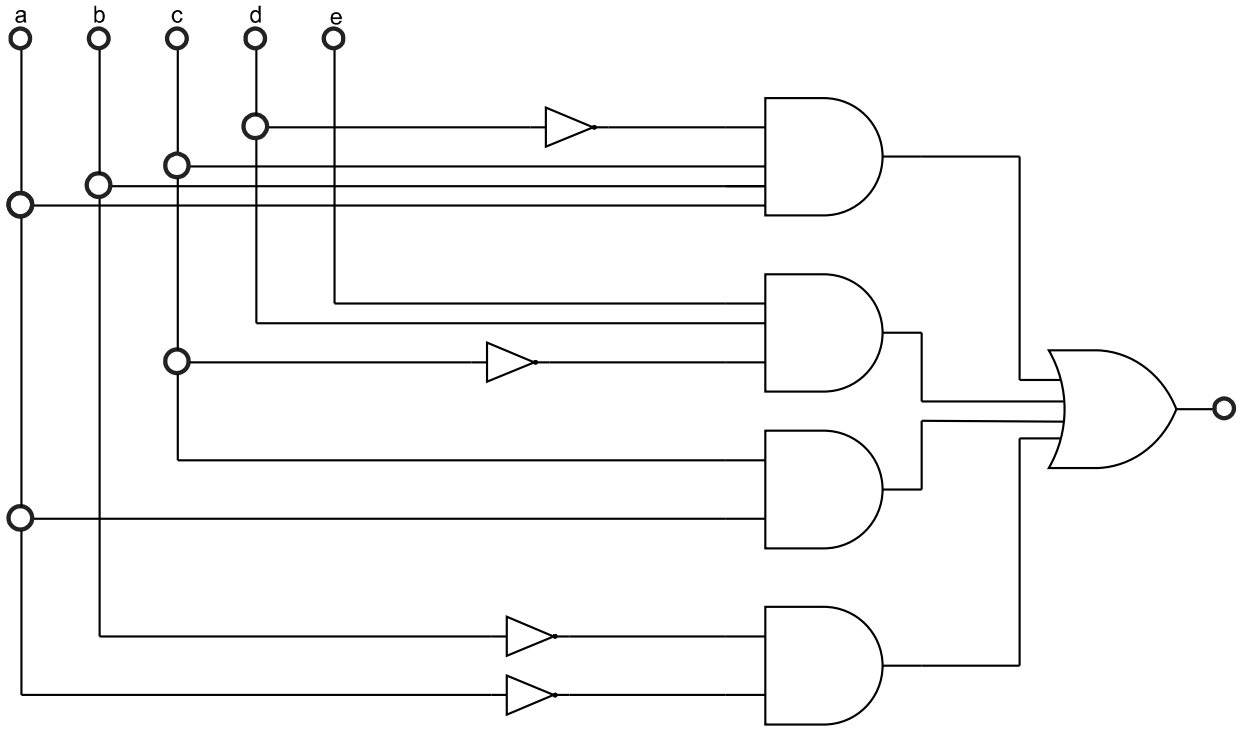
\includegraphics[width=0.9\textwidth]{Circuito1.PNG}
\caption{Circuito resultante de simplificar la expresión (\ref{equ:minterms}).}
	\label{fig:circ1}
\end{figure}

Por otro lado, para la expresión (\ref{equ:maxterms}) se escribe en forma de maxterminos:

\[
	f \left( d,c,b,a \right) = \left( a + b + c + d \right) \cdot \left( a + \bar{b} + c + d\right) \cdot \left( a + b+ \bar{c} + d \right) \cdot \left( \bar{a} + \bar{b} + \bar{c} + d \right) \cdot
\]
\[
	\left( a + b + c + \bar{d} \right) \cdot \left( a + \bar{b} + c + \bar{d} \right) \cdot \left( a + b + \bar{c} +\bar{d} \right)
\]

\begin{centering}
    \begin{Karnaugh}
        \minterms{1,3,5,6,9,11,13,14,15}
        \maxterms{0,2,4,7,8,10,12}
        
        \implicant{0}{8}{yellow}
        \implicantcantons{red}
        
    \end{Karnaugh}
\par\end{centering}


\begin{table}[H]
\centering
\caption{Mapa de Karnaugh de la expresión (\ref{equ:maxterms}).}
\label{tabla:maxterms}
\end{table}

En esta se pueden observar 3 grupos:
\begin{enumerate}
	\item Compuesto por los casilleros 0, 4, 8 y 12, obteniéndose la expresión $ b + a $;
	\item Compuesto por el casillero 7, obteniéndose la expresión $ \bar{a} + \bar{b} + \bar{c} + d $;
	\item Compuesto por los casilleros 0, 2, 8 y 10, obteniéndose la expresión $ c + a $
\end{enumerate}

obteniendo finalmente la expresión: 

\begin{equation}
	f \left( d,c,b,a \right) = \left( b \ + \ a \right) \cdot \left( c \ + \ a \right) \cdot \left( \bar{a} \ + \ \bar{b} \ + \ \bar{c} \ + \ d \right)
\end{equation}

\begin{figure}[H]
	\centering
	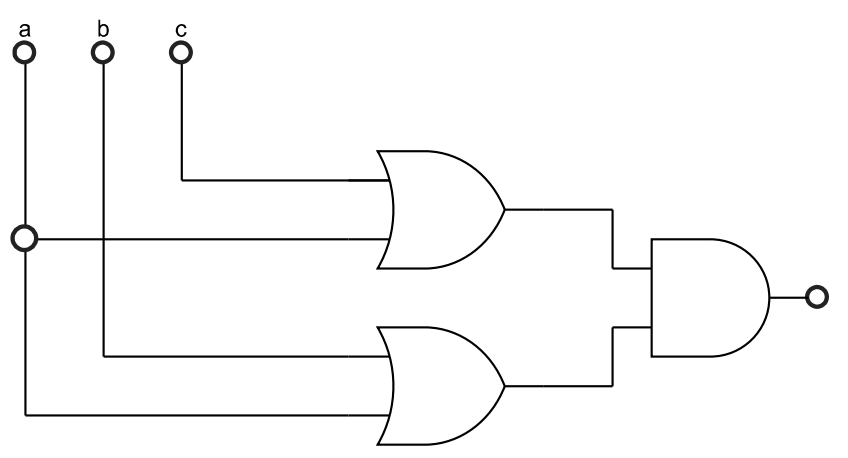
\includegraphics[width=0.9\textwidth]{Circuito2.PNG}
\caption{Circuito resultante de simplificar la expresión (\ref{equ:maxterms}).}
	\label{fig:circ2}
\end{figure}


\section*{Conclusión}


\end{document}
